\chapter{Results}
\label{chapter:Results}

\begin{introduction}
    "The only source of knowledge is experience." - Albert Einstein
\end{introduction}

\section{Evolution of Software Development}

The software development process has undergone several important stages, each enhancing its functionality and usability. The figures below illustrate the application's progress, showcasing different phases of refinement as the project matured.

\subsection{Initial Stages: Basic Functionality and User Interaction}

The first figure (Figure \ref{fig:v1}) represents the early stages of development, where the primary focus was on creating a user-friendly interface for calculating average read depth and coverage metrics at diferent threshold from a BAM file for a Single Gene. In this version, the application prominently features a two-step process where the user selects a BED file releated to the gene to analyse and one or more BAM files. These files are then processed to calculate key metrics, which are displayed in the results table below. This simple design allowed for efficient user interaction but was somewhat limited in terms of flexibility and scope.

At this stage, the core challenge was to ensure that the software could handle large genomic files while presenting the results in a clear and intuitive format. The layout emphasizes simplicity, making it easier for users to navigate through the two-step process. However, as the project progressed, the need for more advanced features became evident.

\begin{figure}[H]
    \centering
    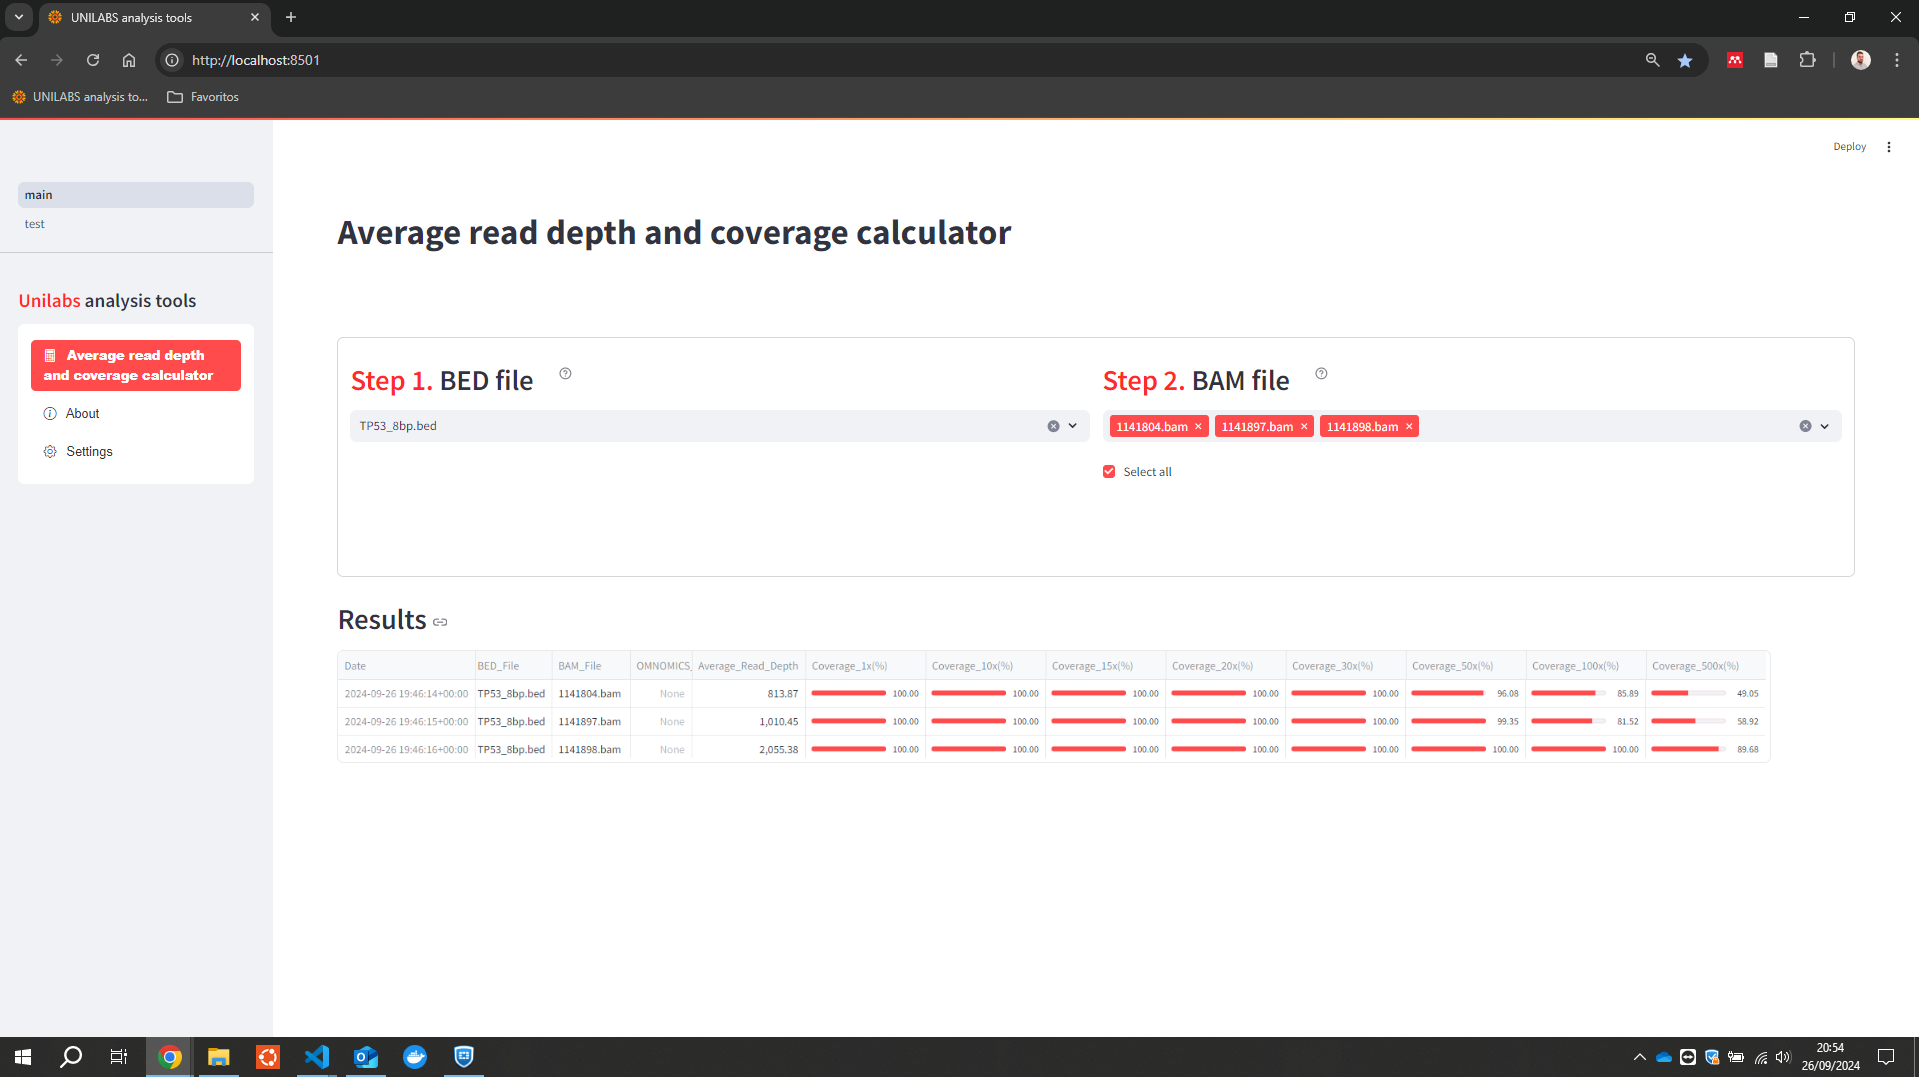
\includegraphics[width=1\textwidth]{figs/v1.png}
    \caption{First version of the GUI.} 
    \label{fig:v1}
\end{figure}

\subsection{Refinement: Introducing Flexibility and Multiple Analysis Modes}

In the second figure (Figure \ref{fig:v2}), the software has significantly evolved to include more detailed analysis options. The interface now presents multiple analysis types: \textit{Single Gene}, \textit{Gene Panel}, and \textit{Exome}, catering to different research needs. This flexibility represents a major shift from the earlier version, as it now allows users to select specific genome assemblies and regions of interest by using an universal BED file. Additionally, the results section has been split into tabs such as \textit{Overview} and \textit{Exon Details}, giving users the ability to drill down into the metrics for a the gene or explore exon-level coverage details. However, even though this last features were thinked to be used in this version, they only have been work fully in the last version of the software.

\begin{figure}[H]
    \centering
    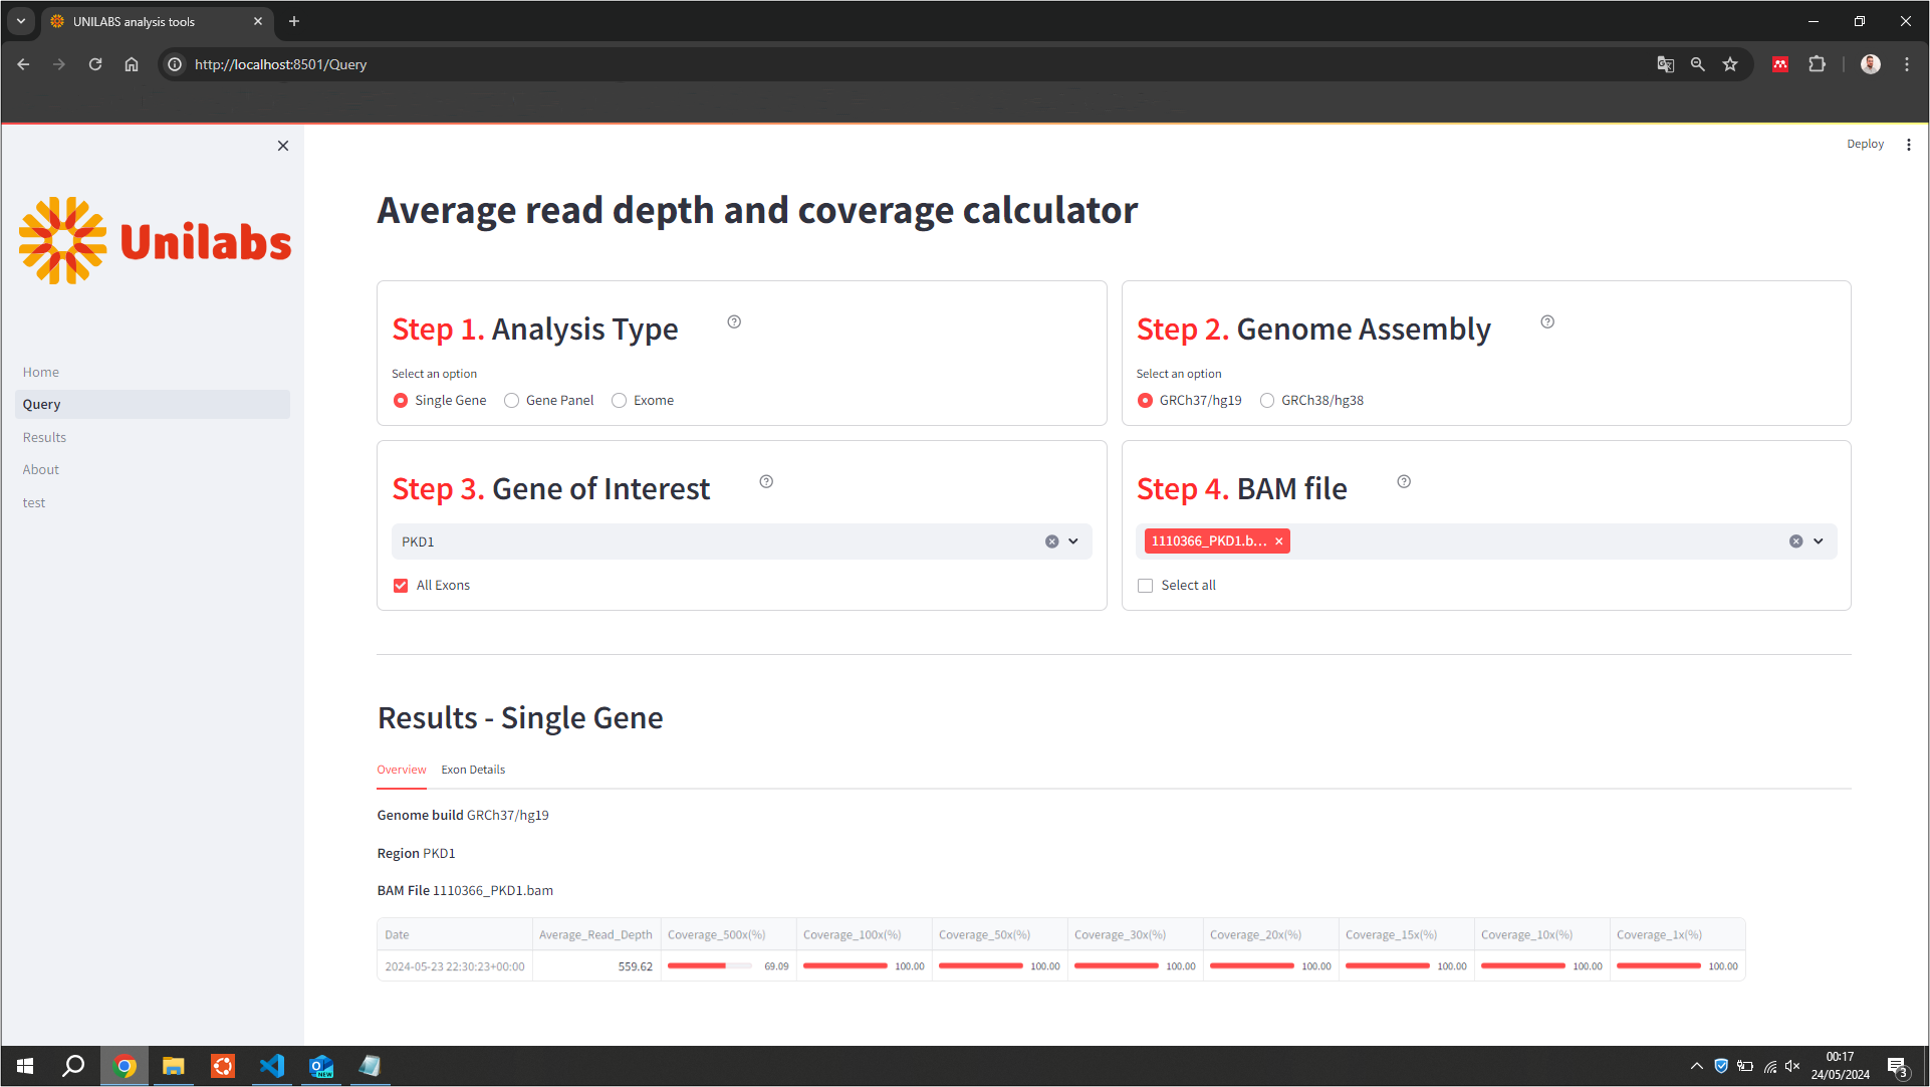
\includegraphics[width=1\textwidth]{figs/v2.png}
    \caption{Second version of the GUI.} 
    \label{fig:v2}
\end{figure}


The final version of the software is presented in the next section in detail with real-world data to showcase its full capabilities and effectiveness in genomic analysis. This final iteration represents the culmination of numerous improvements in both the user interface and the backend computational logic, making it a powerful tool for researchers.

\subsection{Overview of the Final Version}

The final version of the software maintains the core functionality established in earlier versions, such as calculating average read depth and coverage metrics from BED and BAM files. However, it has evolved to include more refined features, enhanced performance, and the ability to handle more complex datasets.

This section presents a detailed overview of the final version of the software using real-world genomic data, illustrating its capabilities in calculating read depth and coverage for genomic regions of interest. The images provided demonstrate the final interface and processing stages.

\subsubsection{\textbf{Login Interface}}

As seen in Figure \ref{fig:login}, the software begins with a user authentication process, offering a simple and clean login interface. This feature, although optional in the final deployment, ensures that access to sensitive data is controlled. Users must input their credentials, and upon successful authentication, they are granted access to the full range of analysis tools.

\begin{figure}[H]
    \centering
    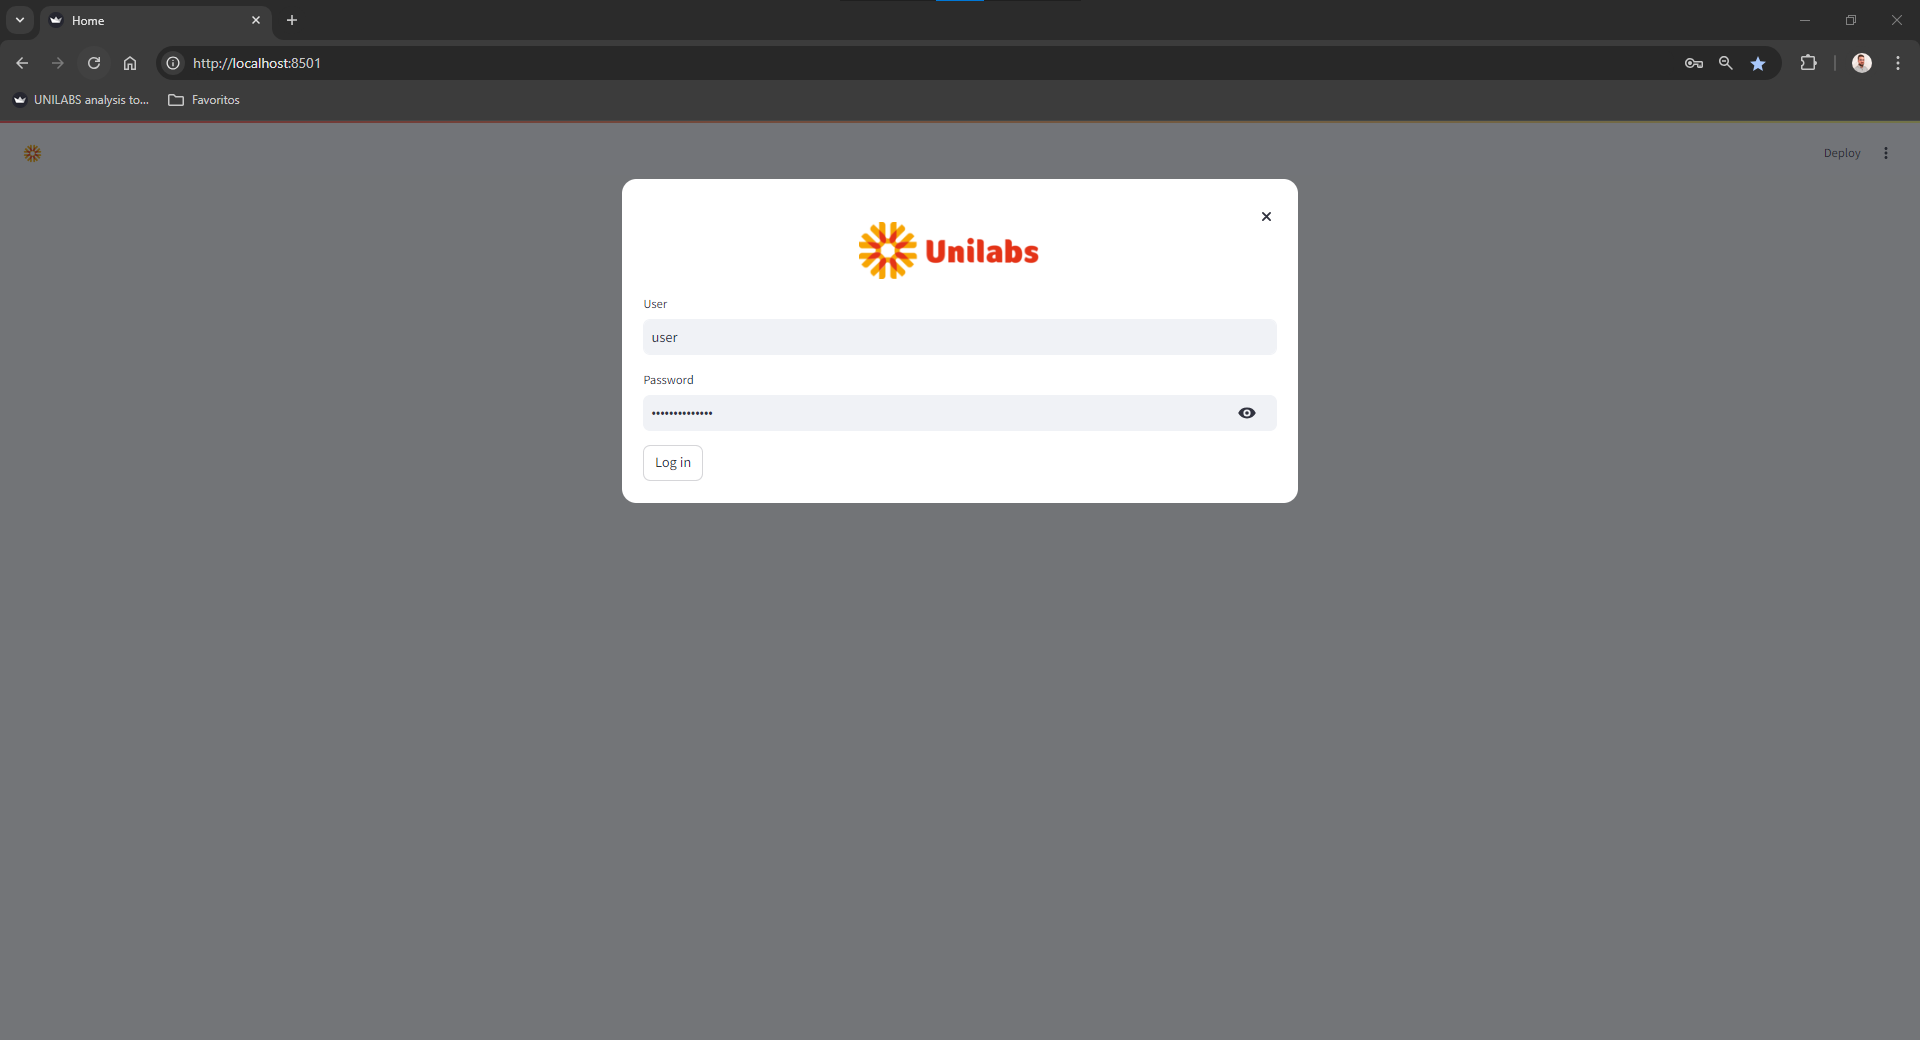
\includegraphics[width=\textwidth]{figs/v3.1.png}
    \caption{Login Interface for the Software}
    \label{fig:login}
\end{figure}

The next step of the process involves selecting the analysis type, as shown in Figure \ref{fig:single_gene}. Users can choose between three options: Single Gene, Gene Panel, and Exome. This selection determines the scope of the analysis and the subsequent steps in the workflow.


\subsubsection{\textbf{Single Gene Analysis}}

In this version, users can perform a single gene analysis by selecting the appropriate options for genome assembly and gene of interest. The software also provides the option to analyze all exons within the selected gene or focus on specific exons of interest. BAM/CRAM files containing the sequencing data are acessed and processed by samtools for detailed metrics.

\begin{figure}[H]
    \centering
    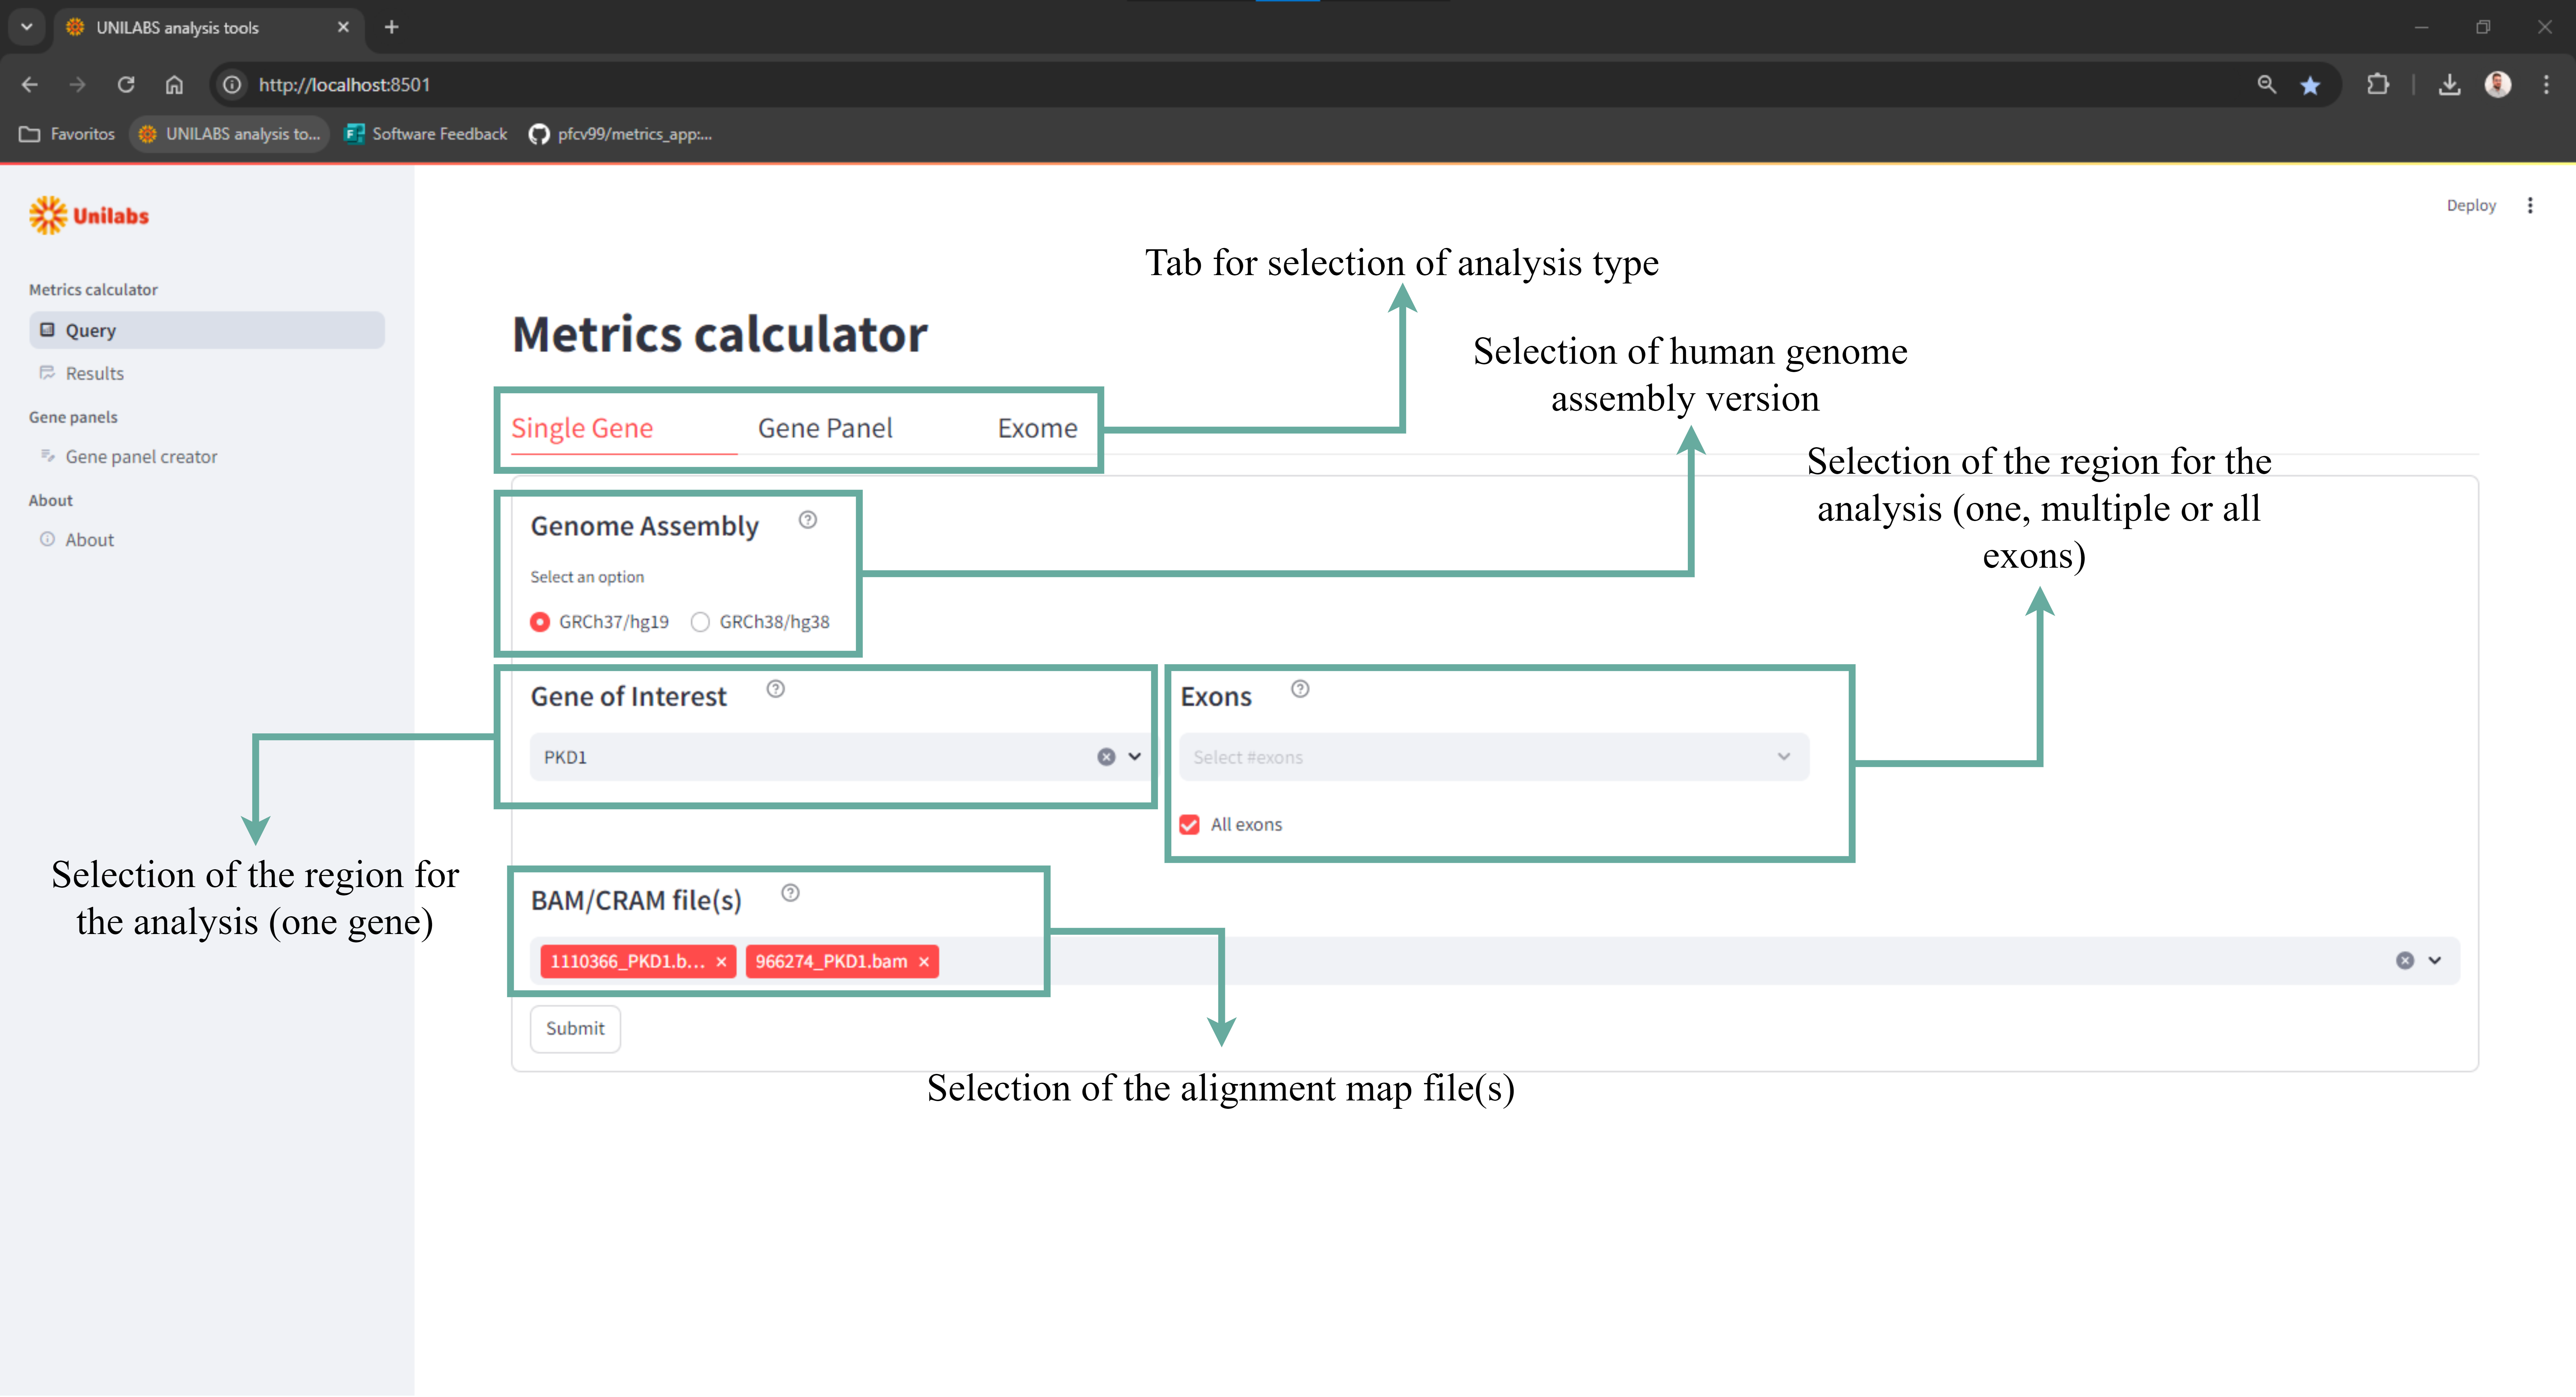
\includegraphics[width=\textwidth]{figs/v3.2.png}
    \caption{Single Gene Analysis Workflow}
    \label{fig:single_gene}
\end{figure}

\begin{itemize}
    \item \textbf{Results and Report Generation}

    Once the data is processed, users can access the results in the 'Results' tab, as seen in Figure~\ref{fig:results_loading}. The software compiles a detailed report that includes various metrics such as average read depth, breadth of coverage, and coverage percentages across different thresholds (e.g., 10x, 20x, 30x). This data is also available for download in a PDF format, ensuring users can retain a permanent copy of the analysis results.
    
    \begin{figure}[H]
        \centering
        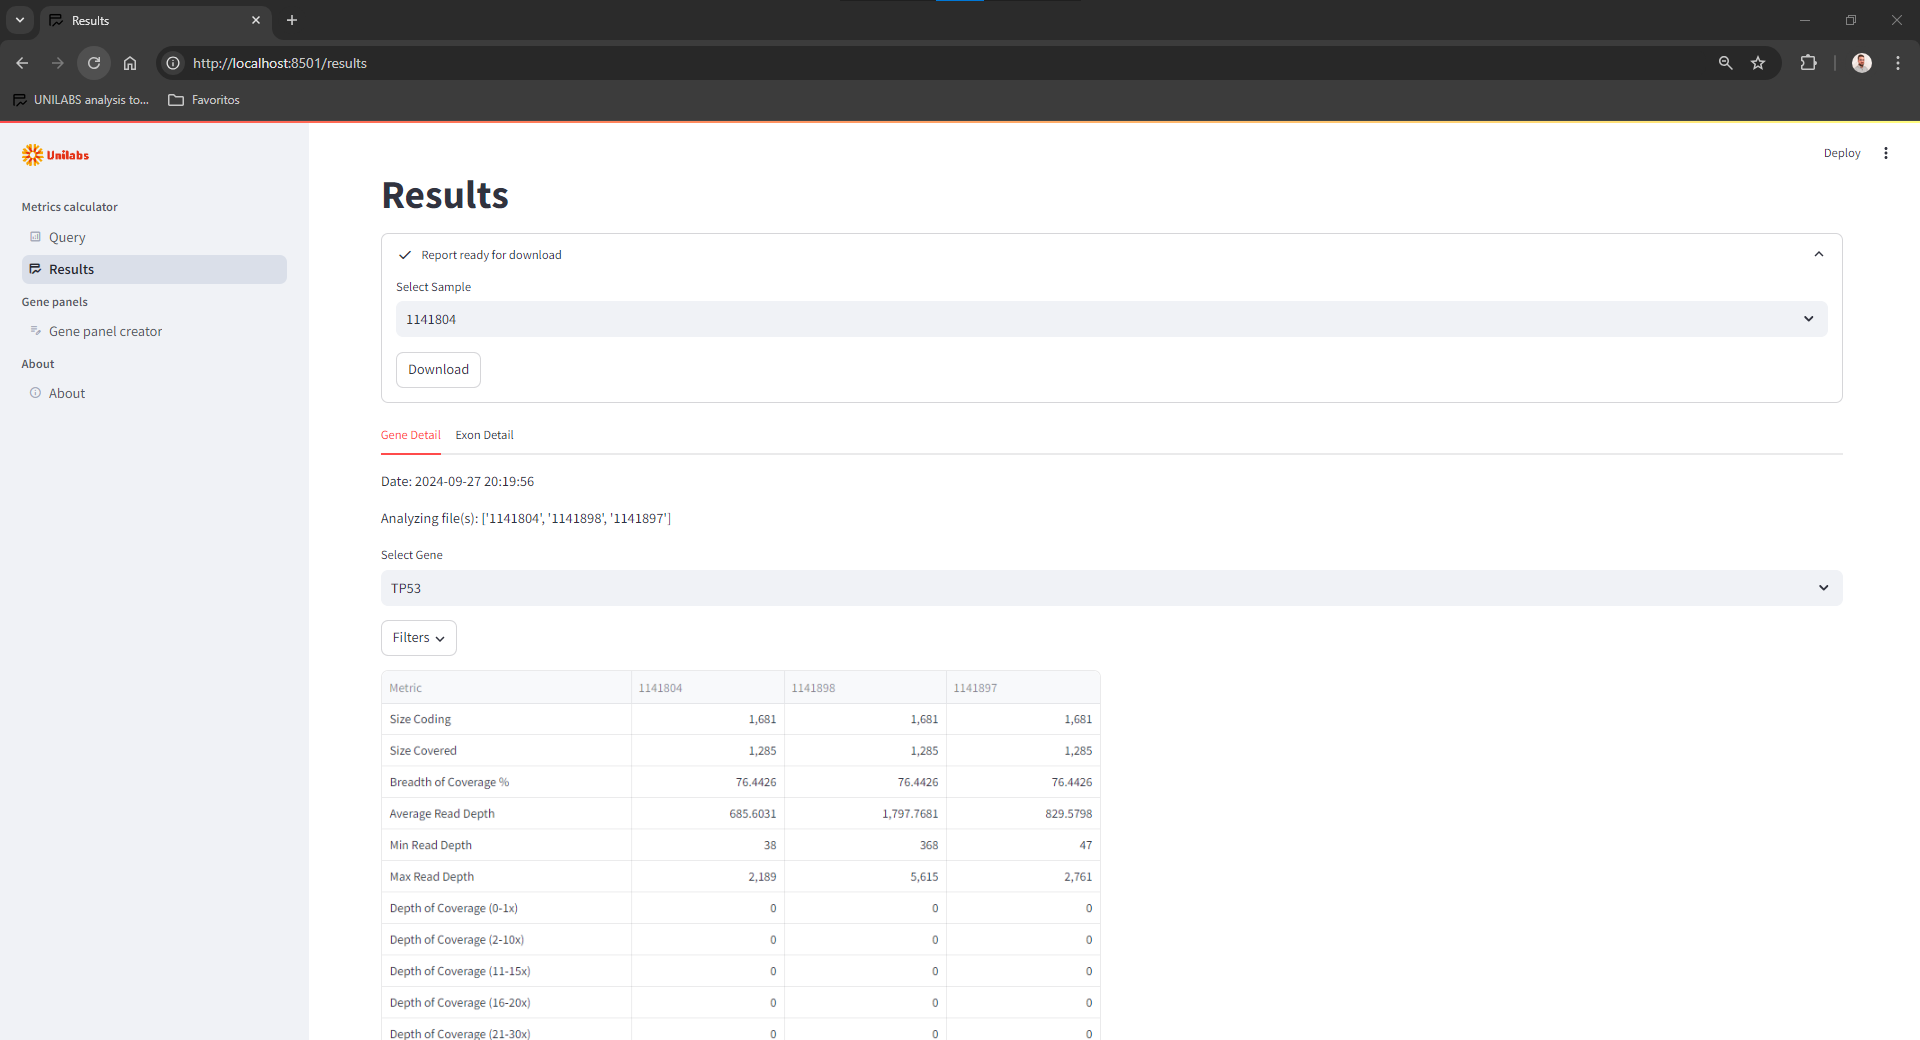
\includegraphics[width=\textwidth]{figs/v3.3.png}
        \caption{Results Tab Loading the Final Report}
        \label{fig:results_loading}
    \end{figure}
    
    In Figure \ref{fig:results_loading} and \ref{fig:final_report}, the detailed metrics for the gene \textit{TP53} are displayed, offering both gene-level and exon-level statistics. This comprehensive breakdown allows researchers to thoroughly assess the sequencing coverage for the analyzed samples. Key metrics include the size coding of the gene, minimum and maximum read depth, and coverage percentages across various depth thresholds, providing valuable insights into the quality and completeness of the sequencing data.
    
    For this case study, the size coding of the \textit{TP53} gene is 1,681 base pairs (bp), with a covered size of 1,285 bp for all three samples, resulting in a Breadth of Coverage of 76.4\%. The average read depth across the three samples was 685.6x, 1,797.8x, and 829.6x, respectively. Sequencing depth, or the number of times a particular region of the genome is covered by reads, directly impacts the reliability of variant detection, gene expression studies, and other genomic analyses. Inconsistent or insufficient depth may lead to variability in the ability to accurately detect mutations or copy number variations, potentially resulting in false positives or false negatives. For instance, lower depth may miss variants that are present at low frequencies, while higher depth ensures that even rare mutations are confidently identified. \cite{Larson2023}
    
    When examining the depth of coverage across different thresholds, the coverage percentages for the 10x, 20x, and 30x thresholds were consistently 100\% for all three samples, demonstrating that all regions of interest achieved sufficient coverage at these lower thresholds. However, at higher thresholds, the depth of coverage showed more variability. For the 50x threshold, the coverage percentages were 95.3\%, 100\%, and 99.2\%, respectively. Similarly, at the 100x threshold, the coverage percentages were 83.8\%, 100\%, and 78.5\%. Finally, at the highest threshold of 500x, the coverage percentages dropped more significantly, with values of 41.4\%, 88.2\%, and 52.8\%, respectively.
    
    \begin{figure}[H]
        \centering
        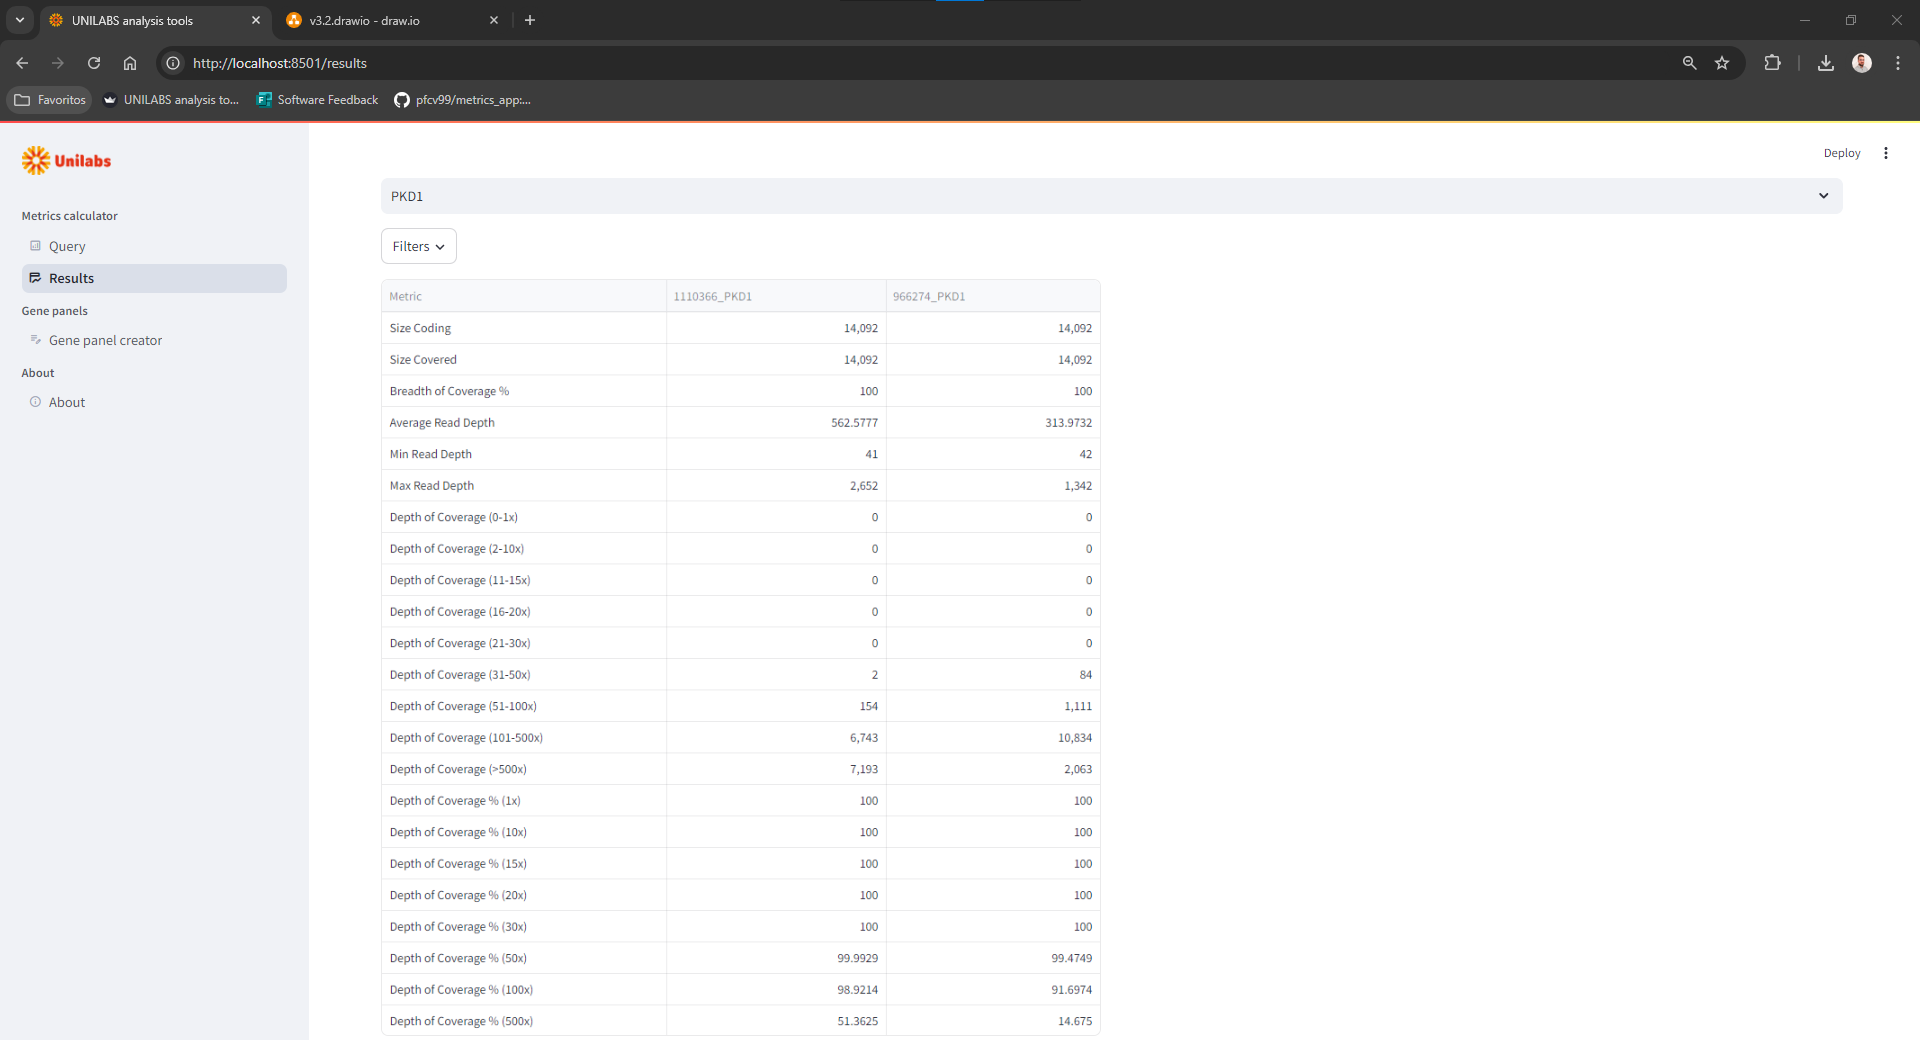
\includegraphics[width=\textwidth]{figs/v3.4.png}
        \caption{Final Report with Detailed Metrics for Gene TP53}
        \label{fig:final_report}
    \end{figure}
    
    \item \textbf{Depth of Coverage Visualization}
    
    One of the critical features of the final software version is its ability to visualize depth of coverage, as shown in Figure \ref{fig:coverage_plot}. This visualization allows users to see the depth of sequencing across the gene of interest, with blue regions highlighting exons. A threshold can be set by the user, and regions that fall below this threshold are highlighted in red, ensuring that gaps or low-coverage areas are easily identified. This is particularly important for researchers assessing the completeness of their sequencing data.
    
    \begin{figure}[H]
        \centering
        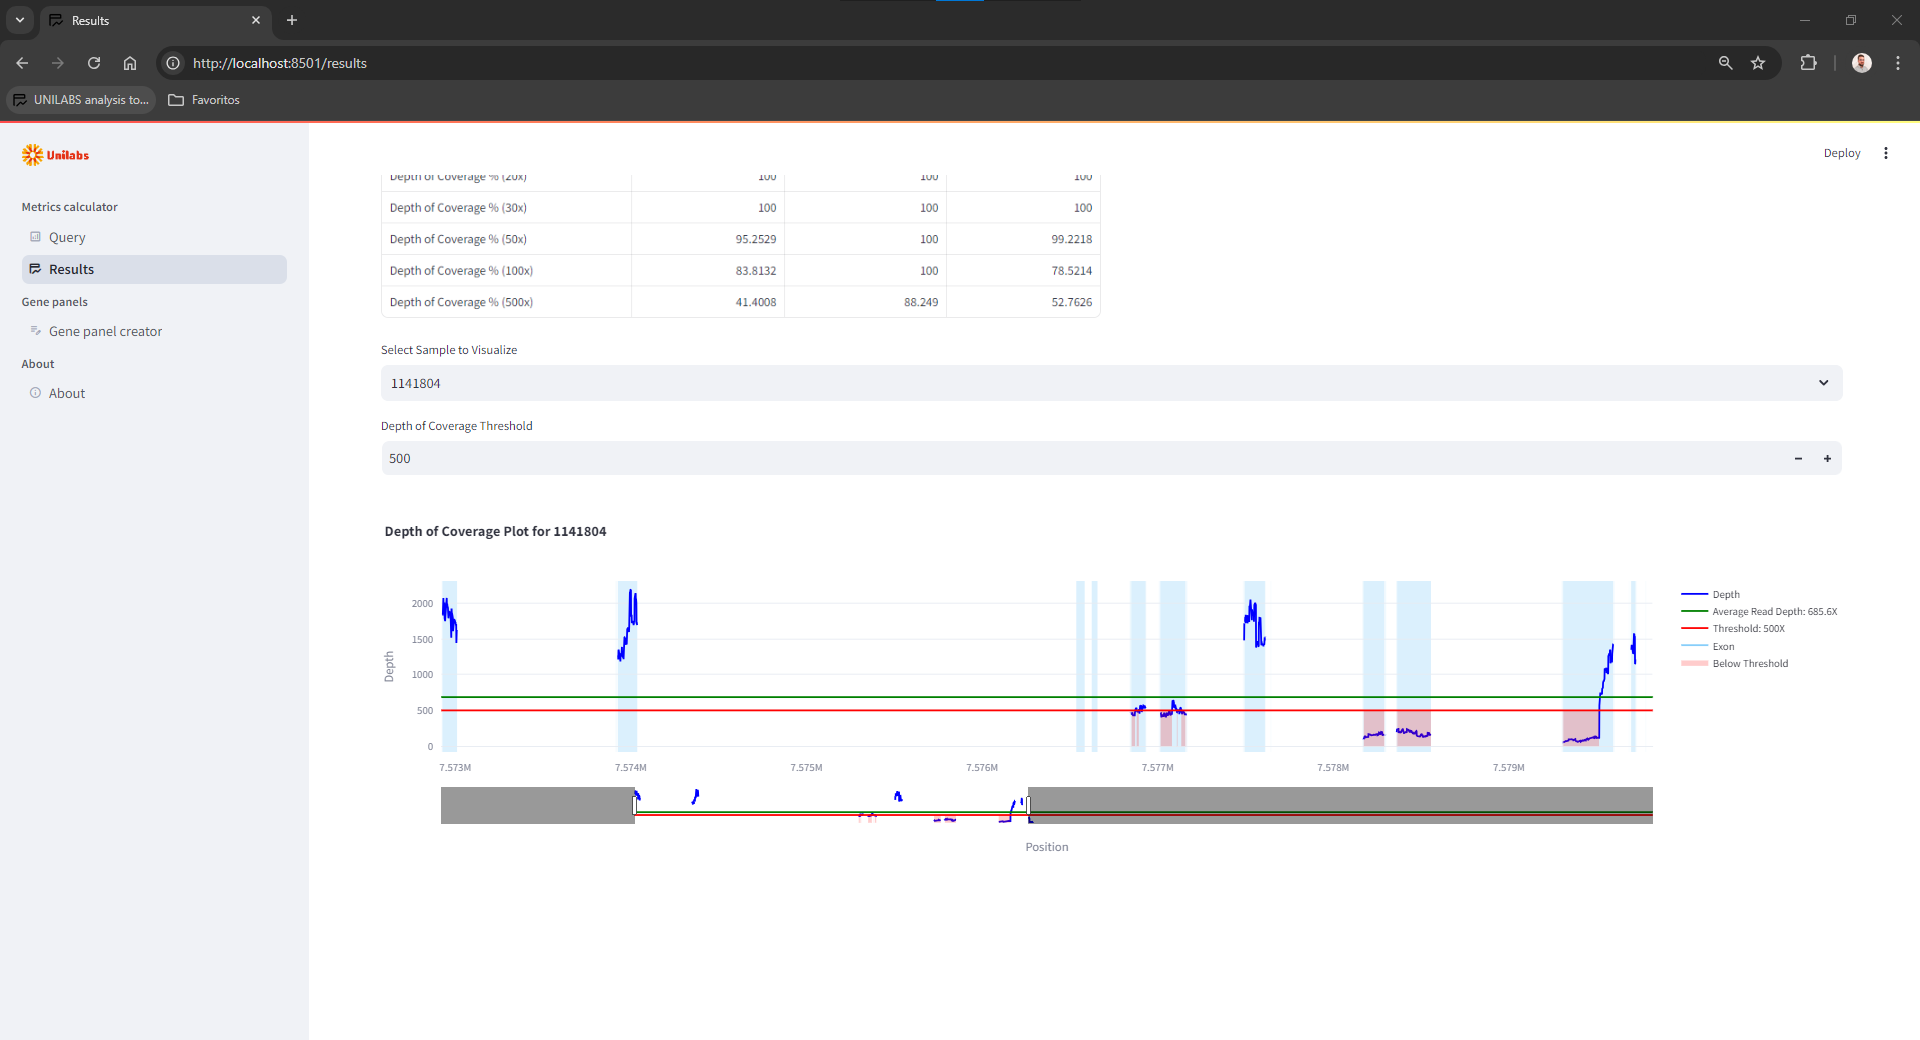
\includegraphics[width=\textwidth]{figs/v3.5.png}
        \caption{Depth of Coverage Visualization for Gene TP53}
        \label{fig:coverage_plot}
    \end{figure}
\end{itemize}

\subsubsection{\textbf{Gene Panel Analysis}}


In the gene panel analysis, the software is configured to process multiple genes simultaneously, as opposed to the single gene analysis. This functionality is particularly useful when studying gene panels associated with specific hereditary diseases, such as the BRCA1 and BRCA2 genes, commonly linked to breast and ovarian cancer. The analysis workflow is similar to that of a single gene but extends to multiple regions of interest, providing broader insights into the coverage and depth across the entire panel.

\begin{itemize}
\item \textbf{Panel Selection and Input}

The user begins by selecting the appropriate genome assembly and the gene panel of interest. For this case study, the panel for hereditary breast and ovarian cancer was selected, which includes the BRCA1 and BRCA2 genes. The input consists of a BAM or CRAM file associated with the selected panel, as shown in Figure \ref{fig:panel_input}.

\begin{figure}[H]
    \centering
    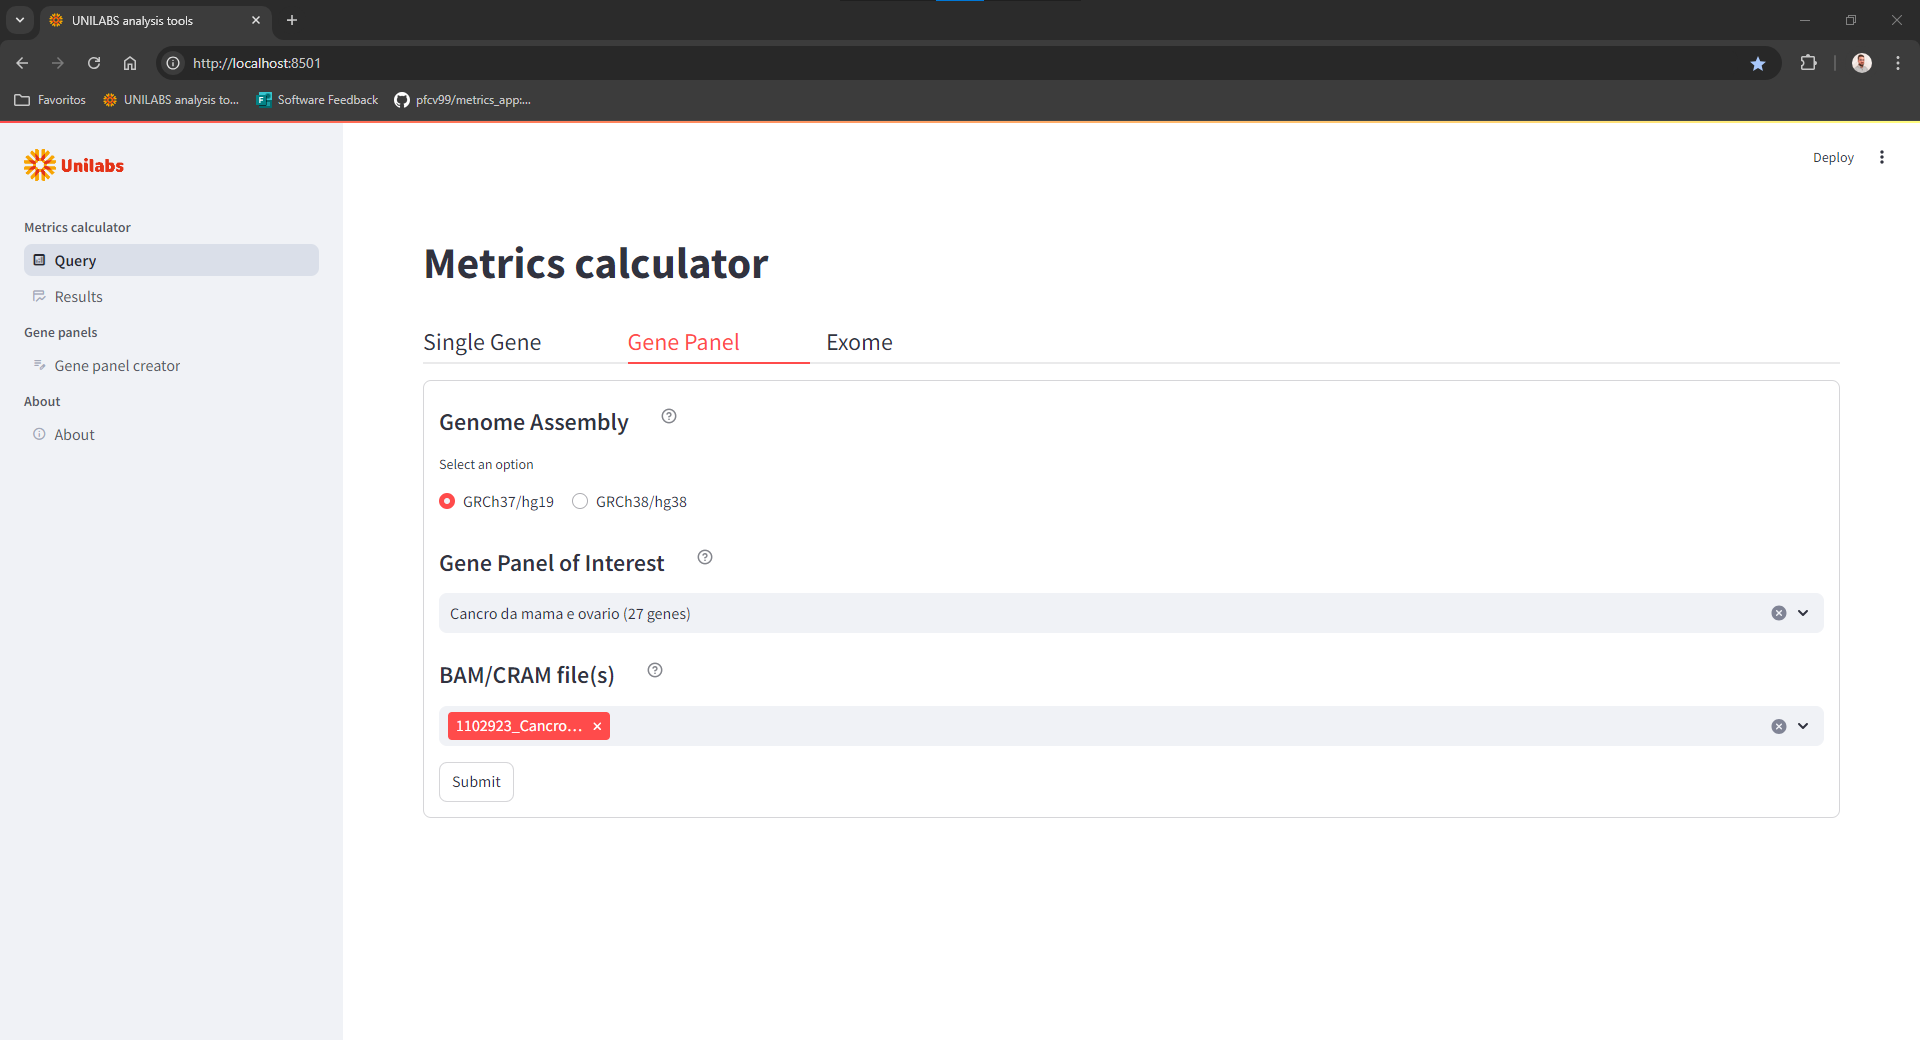
\includegraphics[width=\textwidth]{figs/v3.8.png}
    \caption{Gene Panel Input Selection and Submission}
    \label{fig:panel_input}
\end{figure}

\item \textbf{Overall Results for the Gene Panel}

Once the data is processed, the software generates a comprehensive table of metrics for the entire gene panel. This includes critical metrics such as size coding, size covered, breadth of coverage, and average read depth. These metrics are essential for evaluating the quality of sequencing across all genes in the panel. Figure \ref{fig:panel_results_overall} illustrates the results generated for the gene panel associated with hereditary breast and ovarian cancer. For this specific panel, for a panel with a size coding of 17.080 base pairs (bp), the size covered was 16.735 bp, resulting in a Breadth of Coverage of 97.99\%. The average read depth across the panel was 294.2x, with a minimum read depth of 1x and a maximum read depth of 533x. The depth of coverage across different thresholds revealed that the panel achieved a coverage between 99.8\% and 100\% at the 10x, 20x, and 50x thresholds, and 97.8\% at the 100x threshold. For the 500x threshold, the coverage percentage dropped to 0.6\%, indicating regions with lower depth of coverage. 

\begin{figure}[H]
    \centering
    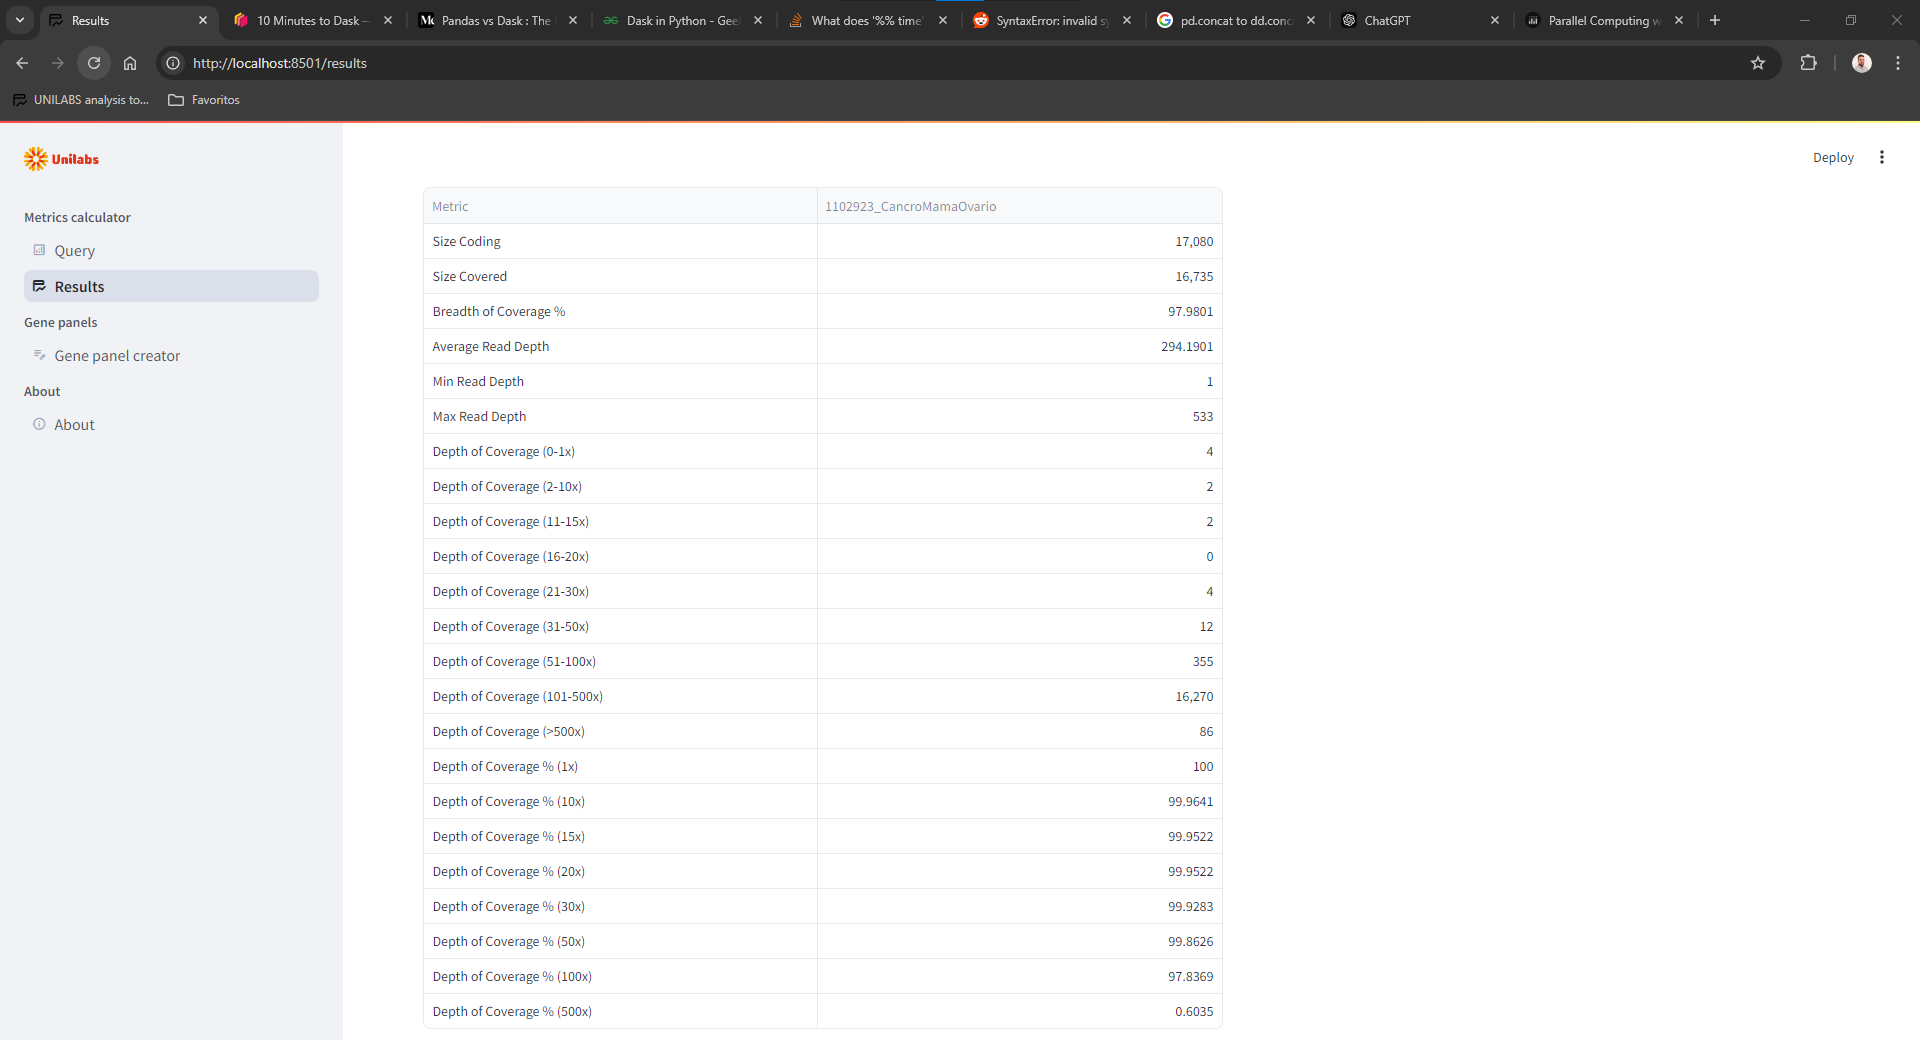
\includegraphics[width=\textwidth]{figs/v3.9.png}
    \caption{Overall Gene Panel Results for Hereditary Breast and Ovarian Cancer}
    \label{fig:panel_results_overall}
\end{figure}

\item \textbf{Individual Gene Metrics}

The software allows users to dive deeper into the metrics for individual genes within the panel. Figures \ref{fig:brca1_results} and \ref{fig:brca2_results} display the results for the BRCA1 and BRCA2 genes, respectively. The size coding of BRCA1 was 6343 base pairs (bp), with a covered size of 6124 bp, resulting in a Breadth of Coverage of 96.5\%. The average read depth for BRCA1 was 345.3x, with a minimum read depth of 1x and a maximum read depth of 533x. The depth of coverage across different thresholds showed consistent coverage percentages above 99\% for the 1x, 10x,, 15x, 20x, 30x, 50x and 100x thresholds, with a slight drop to 1.6\% at the 500x threshold. In other hand, the size coding of BRCA2 was 10.737 base pairs (bp), with a covered size of 10.611 bp, resulting in a Breadth of Coverage of 98.8\%. The average read depth for BRCA2 was 264.7x, with a minimum read depth of 1x and a maximum read depth of 446x. The depth of coverage across different thresholds showed also consistent coverage percentages above 99\% for the 1x, 10x,, 15x, 20x, 30x and 50x thresholds, with a slight drop to 97.6\% at the 100x threshold. In the 500x threshold, the coverage percentage dropped to 0\%.

\begin{figure}[H]
    \centering
    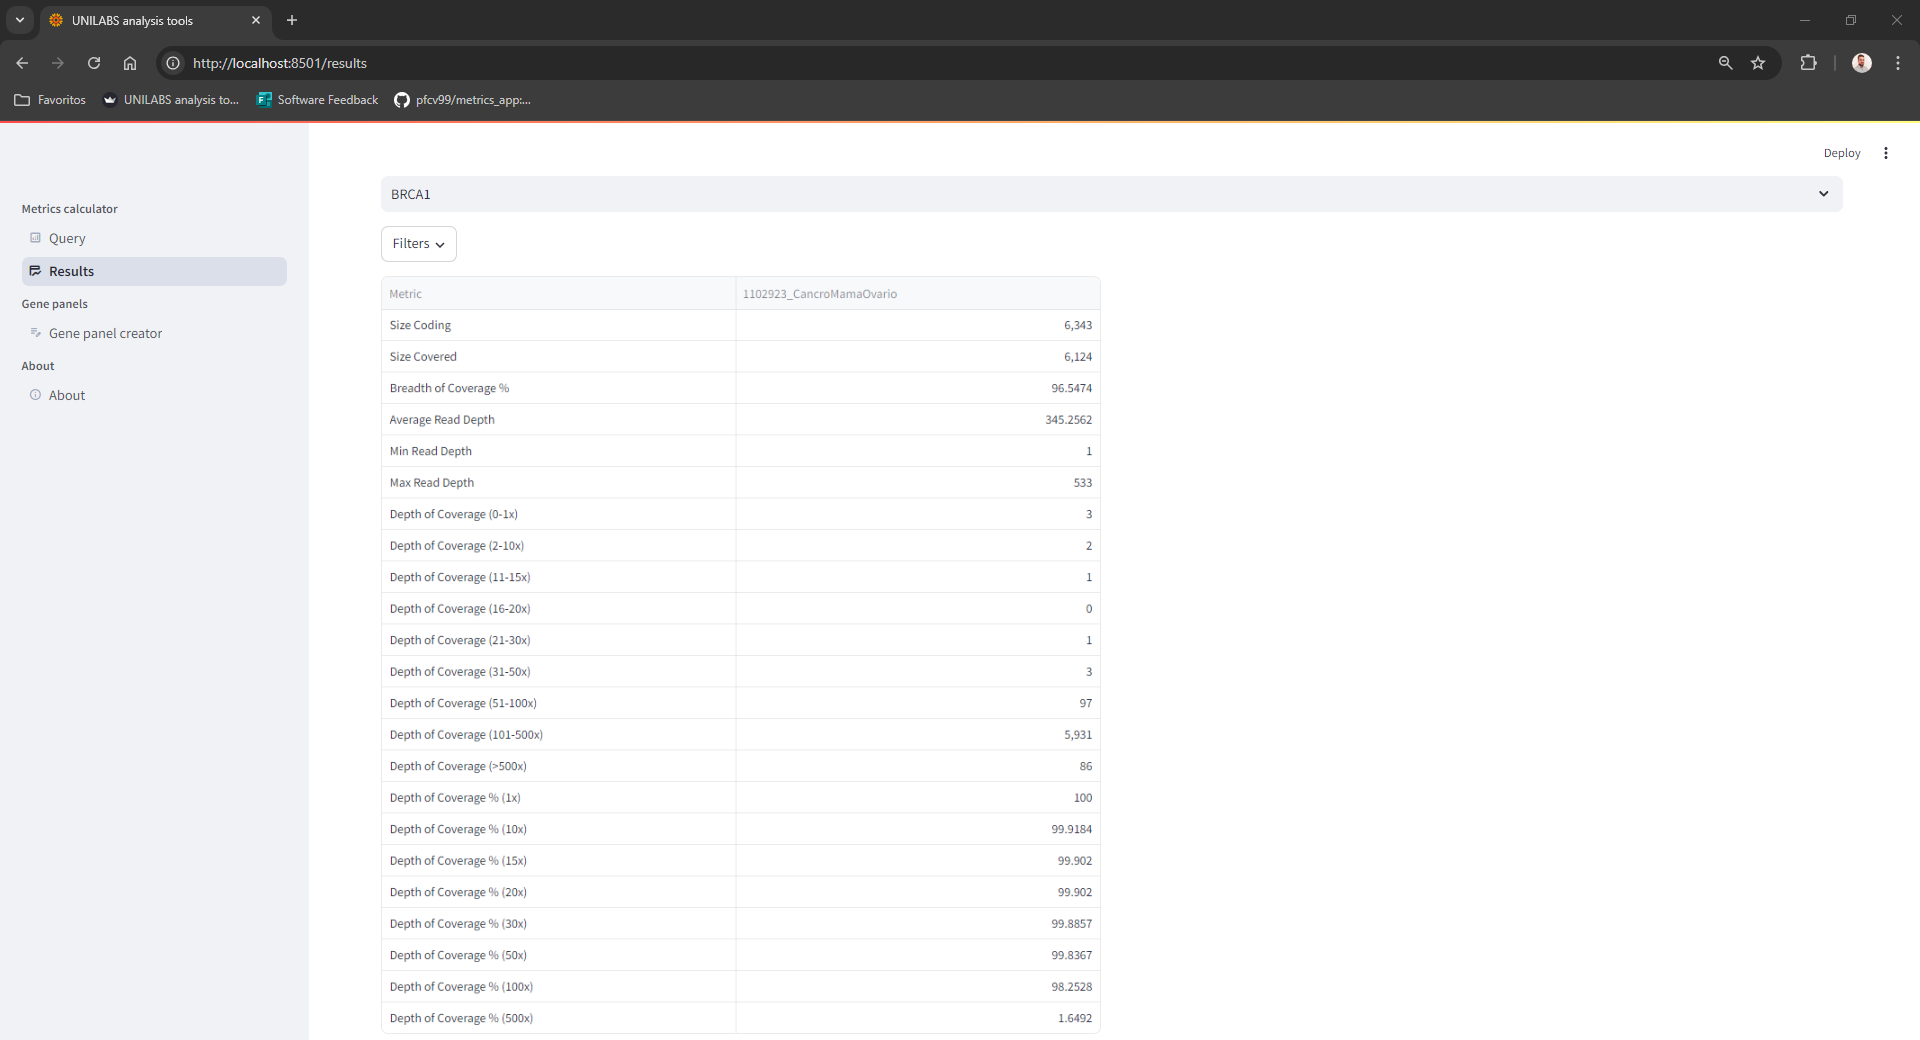
\includegraphics[width=\textwidth]{figs/v3.10.png}
    \caption{Detailed Metrics for the BRCA1 Gene}
    \label{fig:brca1_results}
\end{figure}

\begin{figure}[H]
    \centering
    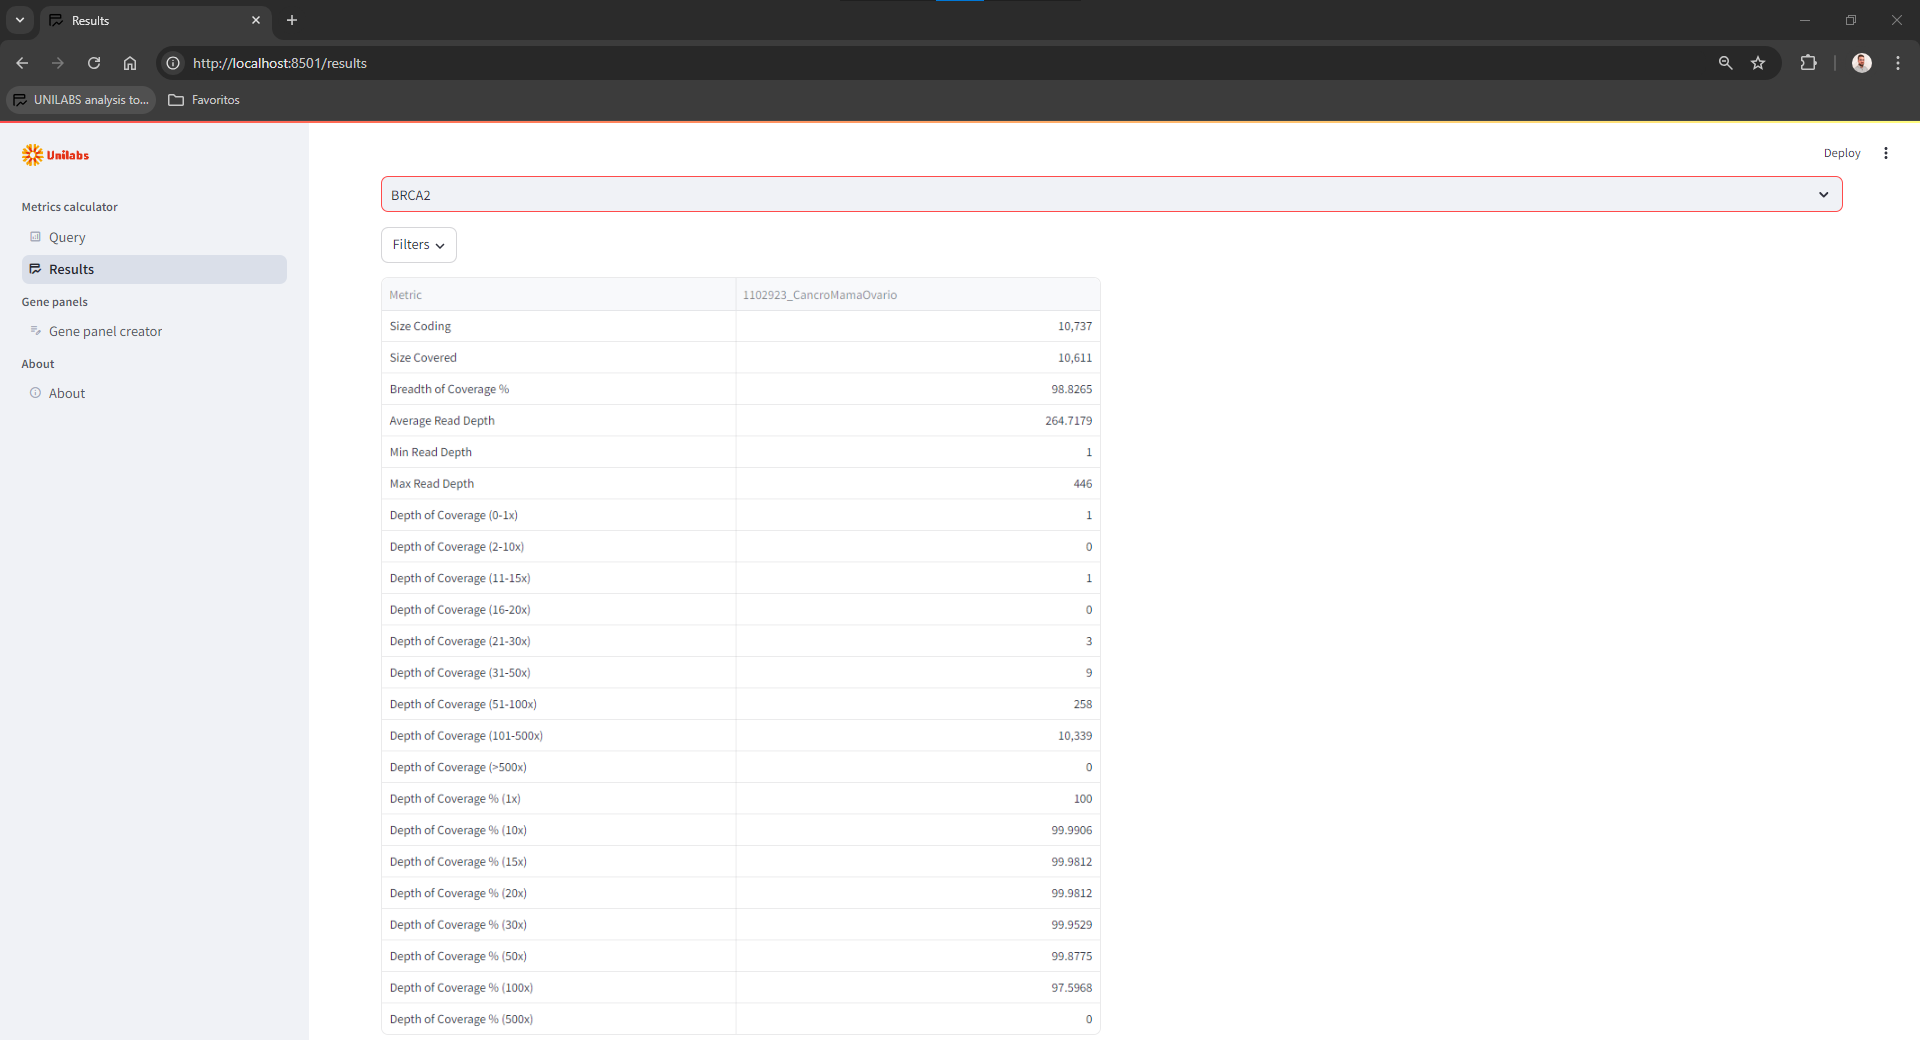
\includegraphics[width=\textwidth]{figs/v3.11.png}
    \caption{Detailed Metrics for the BRCA2 Gene}
    \label{fig:brca2_results}
\end{figure}

\item \textbf{Exon-Level Analysis}

In addition to gene-level metrics, the software also offers exon-level analysis. Users can select specific exons within the genes to obtain a more granular view of the sequencing coverage. This level of detail is particularly useful when assessing the completeness of the sequencing across critical regions within each gene. Figure \ref{fig:exon_results} shows the results for the 124th exon of the BRCA1 gene, where key metrics are also displayed. This exon-level detail allows researchers to pinpoint regions that may require additional sequencing or validation. For the 124th exon of BRCA1, the size coding was 3532 base pairs (bp), with a covered size of 3532 bp, resulting in a Breadth of Coverage of 100\%. The average read depth for this exon was 396.5x, with a minimum read depth of 87x and a maximum read depth of 533x. The depth of coverage across different thresholds showed consistent coverage percentages of 100\% for the 1x, 10x, 15x, 20x, 30x amd 50x thresholds, with a slight drop to 99.1\% at the 100x threshold. In the 500x threshold, the coverage percentage dropped to 2.9\%.

\begin{figure}[H]
    \centering
    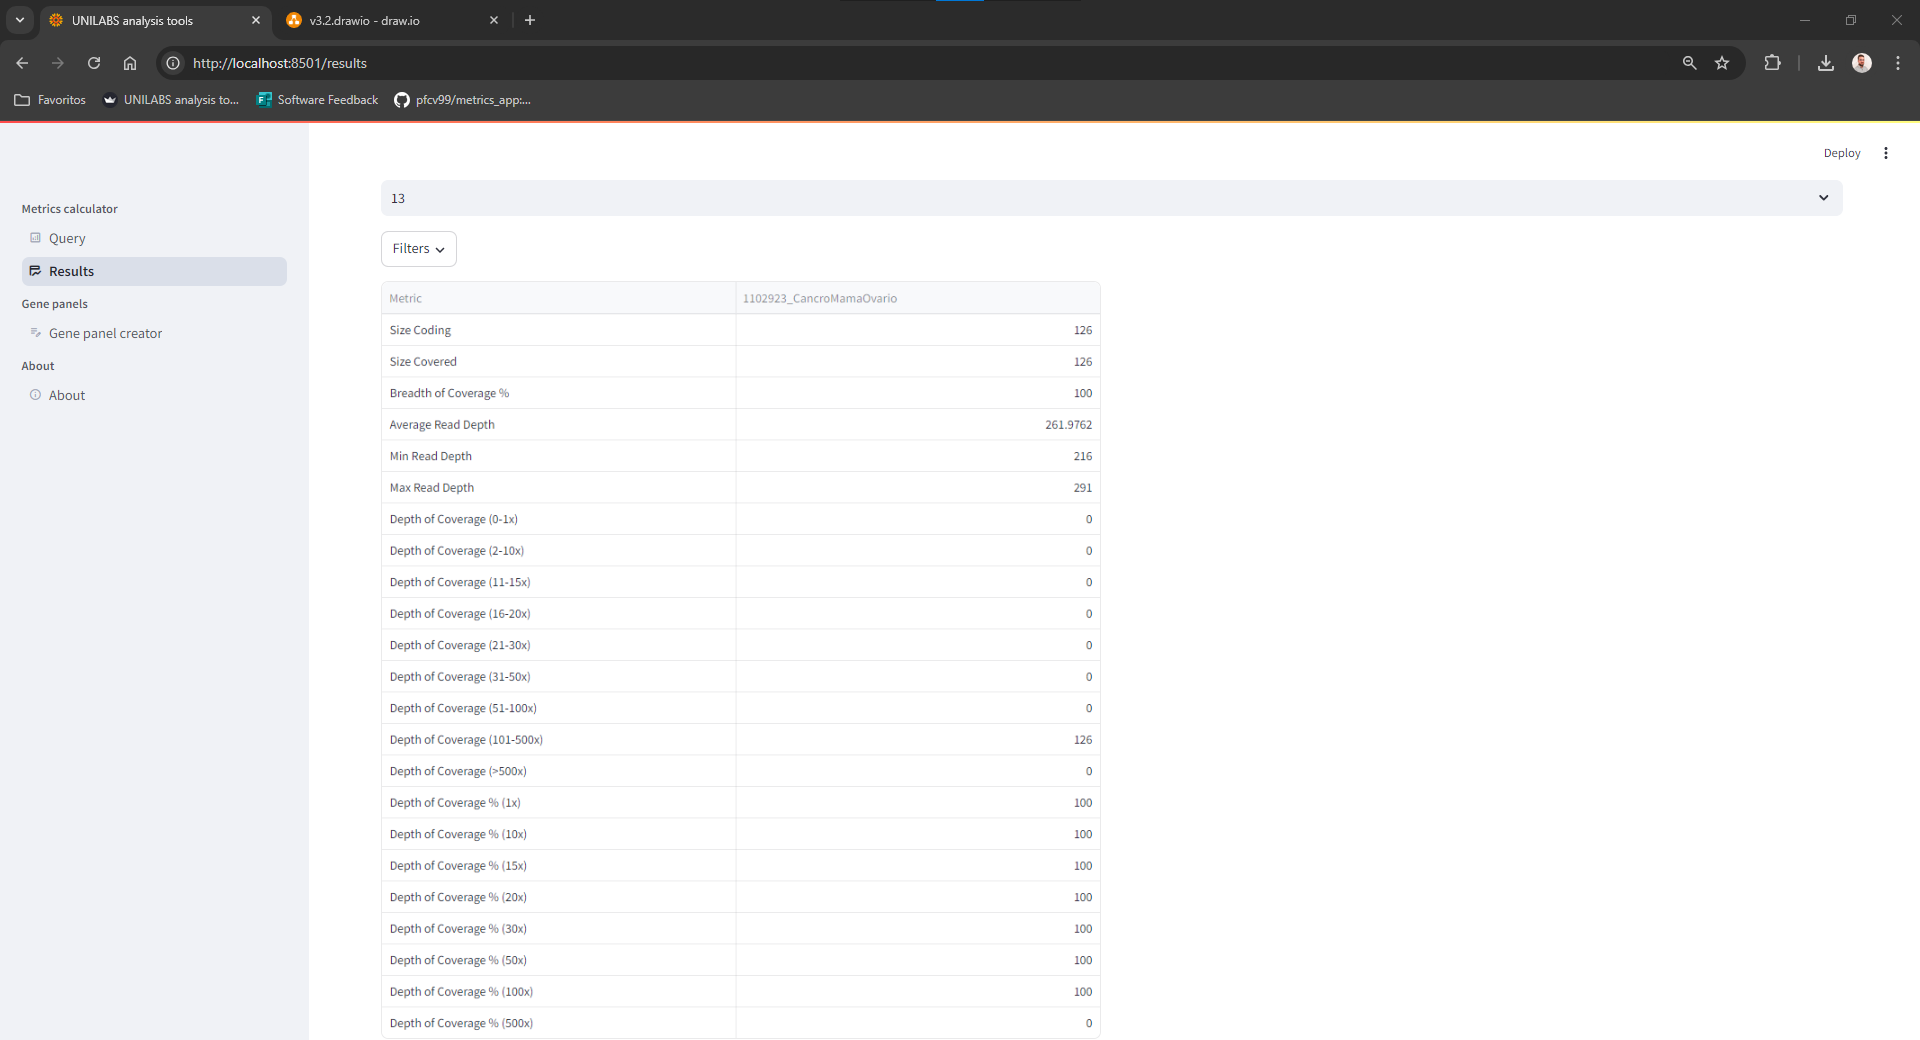
\includegraphics[width=\textwidth]{figs/v3.12.png}
    \caption{Exon-Level Metrics for the BRCA1 Gene}
    \label{fig:exon_results}
\end{figure}

The gene panel analysis feature provides a powerful tool for evaluating sequencing coverage across multiple genes simultaneously. By offering both gene-level and exon-level insights, the software ensures that researchers can thoroughly assess the quality of their sequencing data, identify potential gaps in coverage, and make informed decisions regarding further analysis or re-sequencing.

\end{itemize}

\section{Test and Validation}

To validate the tool, each BAM file was analyzed using the commercial software Omnomics, and the results were compared with those obtained from the developed software. The analyses were performed separately for a Single Gene and a Gene Panel, ensuring that each BAM file was used for its respective analysis.

\subsection{Single Gene Analysis}

The gene TP53 was selected for the Single Gene analysis, and the results obtained from the developed software were compared with those from Omnomics. The metrics compared included Average Read Depth and Depth of Coverage \% (1x, 10x, 20x, 30x, 50x, 100x, 500x).

\begin{table}[]
    \centering
    \caption{Comparison of Metrics between Unilabs Software and Omnomics for Gene TP53}
    \label{tab:omnomicsVSunilabs}
    \begin{tabular}{lrr}
    \textbf{Metric}                      & \textbf{Unilabs Software} & \textbf{Omnomics} \\
    \hline
    Average Read Depth          & 757.20           & 891      \\
    Depth of Coverage \% (1x)   & 100              & 100      \\
    Depth of Coverage \% (10x)  & 100              & 100      \\
    Depth of Coverage \% (20x)  & 100              & 100      \\
    Depth of Coverage \% (30x)  & 100              & 100      \\
    Depth of Coverage \% (50x)  & 100              & 100      \\
    Depth of Coverage \% (100x) & 99.92            & 99.90     \\
    Depth of Coverage \% (500x) & 52.76            & 59      
    \end{tabular}
\end{table}

The comparison of the results between the two software solutions highlights some significant differences. The most notable is in the "Average Read Depth" metric, where the developed software reported an average depth of 757.20, while Omnomics recorded a higher value of 891. This discrepancy is largely attributed to the differences in the reference BED files used by each tool. The developed software utilizes an optimized BED file from Twist by Illumina, whereas Omnomics employs a UCSC Genes BED created using the Table Browser tool from the Genome Browser, specifically targeting the TP53 gene and extending it by 8 base pairs. These differences in BED files lead to variations in the regions covered, directly impacting metrics like read depth.

Both tools reported identical results for the "Depth of Coverage \%" across lower thresholds, such as 1x, 10x, 20x, 30x, and 50x, indicating full coverage for those depths. However, slight deviations emerge at higher coverage thresholds. For example, the "Depth of Coverage \% (100x)" shows almost identical values, with Unilabs Software reporting 99.92\% and Omnomics reporting 99.9\%.

The "Depth of Coverage \% (500x)" shows a more noticeable difference, with Unilabs Software reporting 52.76\%, while Omnomics reported 59\%. This deviation could be explained by the different regions covered by the respective BED files, which affects the depth distribution across the regions analyzed.

While both tools offer highly accurate coverage analyses, the variations in metrics such as Average Read Depth and higher coverage percentages reflect differences in the underlying reference files. The developed software's use of the Illumina Twist BED and Omnomics' reliance on the UCSC Genes BED result in slight but consistent differences, especially in metrics sensitive to the exact regions analyzed.

\subsection{Gene Panel Analysis}

For the analysis of the gene panel "Cancro da mama e ovário (27 genes)", one of the BAM files used was compared between the Unilabs Software and the commercial tool Omnomics. The results are detailed in Table \ref{tab:panel_omnomicsVSunilabs}, highlighting the differences between the two tools for several metrics.

\begin{table}[]
\centering
\caption{Comparison of Metrics between Unilabs Software and Omnomics for Gene Panel: Cancro da mama e ovário (27 genes)}
\label{tab:panel_omnomicsVSunilabs}
\begin{tabular}{lrr}
\textbf{Metric}                      & \textbf{Unilabs Software} & \textbf{Omnomics} \\ \hline
Average Read Depth          & 284.90           & 388      \\
Depth of Coverage \% (1x)   & 100              & 99.60     \\
Depth of Coverage \% (10x)  & 99.26            & 99.50     \\
Depth of Coverage \% (20x)  & 98.96            & 99.40     \\
Depth of Coverage \% (30x)  & 98.87            & 99.20     \\
Depth of Coverage \% (50x)  & 98.39            & 98.80     \\
Depth of Coverage \% (100x) & 95.70            & 96.10     \\
Depth of Coverage \% (500x) & 1.90             & 27.60    
\end{tabular}
\end{table}

The comparison between Unilabs Software and Omnomics for this gene panel reveals several key differences in the reported metrics. Most notably, the "Average Read Depth" shows a significant disparity, with Unilabs Software reporting a depth of 284.9, while Omnomics reports a substantially higher value of 388. This difference can once again be attributed to the different BED files used by each tool. Unilabs Software relies on a Twist BED file provided by Illumina, whereas Omnomics uses a UCSC Genes BED generated through the Table Browser tool in the Genome Browser, specifically targeted for the TP53 gene panel and extended by 8 base pairs. This difference in the reference regions covered affects the distribution of reads across the gene panel, which explains the variance in the reported average read depth.

For the "Depth of Coverage \%" metrics, both tools report similar values, though some minor differences are present. At the 1x coverage threshold, Unilabs Software reports 100\%, while Omnomics reports 99.6\%. Similarly, for the 10x, 20x, 30x, and 50x thresholds, the differences remain small, with Omnomics consistently reporting slightly higher percentages. However, at the 100x threshold, the tools report nearly identical values, with Unilabs Software at 95.70\% and Omnomics at 96.1\%.

The most significant divergence occurs at the 500x threshold. Unilabs Software reports a very low value of 1.90\%, while Omnomics reports a much higher 27.6\%. This discrepancy is likely due to the differing regions targeted by the BED files, with Omnomics potentially including regions of higher coverage within the panel that are not present in the Twist BED file used by Unilabs Software.

Overall, the comparison between the two tools highlights the importance of the reference BED file used in determining coverage metrics. While the results are largely consistent across most coverage thresholds, notable differences, particularly in the average read depth and the highest coverage levels, underscore the impact of BED file selection on the analysis results.

\section{Performance}


\section{Comparison with other tools}


\section{Users feedback}






